
This section describes the current state of the neutrino cross
sections for energies of order of $1$~GeV. Good knowledge of the
neutrino cross section is fundamental in neutrino accelerator
experiment, the introduction of this paragraph explains why. Then, a
summary of the knowledge is made for the nuclear model and the
following processes: charged-current quasi-elastic, resonant, coherent
pion production and deep inelastic scattering. Finally the known
differences between muon and electron (anti-) neutrino scattering are
explained.

\subsection{Introduction}
\label{subsec:xsecintro}
Neutrino cross section predictions are one of the major inputs for any
oscillation experiment; a way to see this is to analyse the equation
that leads to the number of events that are seen in a detector. In the
case of neutrinos, this is:
\begin{equation}
  \label{eq:nevents}
  N(l_\text{rec})=\Phi(E_\text{true})\times \left(1-P(E_\text{true})\right)\times
  \sigma(E_\text{true}, l_\text{true}, A) \times
  \epsilon(l_\text{true})_\text{det} \times R(l_\text{true},
  l_\text{rec})
\end{equation}
where:
\begin{itemize}[noitemsep,topsep=0pt]
\item $N(l_\text{rec})$ refers to the number of events reconstructed
  in a detector in a particular differential bin of a reconstructed
  quantity $l_\text{rec}$ (usually lepton momentum or angle),
\item $\Phi(E_{\text{true}})$ is the flux (which depends on the true energy
  of the neutrino, $E_{\text{true}}$),
\item $P(E_\text{true})$ is the oscillation probability (that also
  depends on the baseline and the oscillation parameters, as seen in
  the Section~\ref{sec:oscillation}),
\item $\sigma(E_\text{true}, l_\text{true}, A)$ is the cross section,
  where $A$ is the target nucleus,
\item $\epsilon(l_\text{true})_\text{det}$ is the detector efficiency,
\item and $R(l_\text{true}, l_\text{rec})$ is the migration matrix (or
  ``smearing matrix'') containing the detector effects to go from
  $l_\text{true}$ to $l_\text{rec}$.
\end{itemize}
Note that this is an approximated equation, since all these quantities
are generally convoluted, rather than simply multiplied.

In most accelerator neutrino oscillation experiments, two detectors
are used; one is next to the neutrino source and measures
$N(l_\text{rec})$ in the special case where the oscillation
probability is zero and the second detector, far from the neutrino
source, measures the same quantity with a non-trivial oscillation
probability.

From the near detector measurement, one can extract a data-driven
constraint on the flux and~/~or the cross section. There are different
ways of doing this:
\begin{itemize}[noitemsep,topsep=0pt]
\item via a direct fit to the flux and cross section as
  is done in \Gls{TK} (as will be seen in Chapter~\ref{chap:banff}),
\item or by directly correcting the true neutrino energy and thus
  modifying the flux ({\it \`a la}
  \Gls{NOvA}~\cite{PhysRevLett.118.231801}).
\end{itemize}

Whichever method is used, the neutrino flux is then extrapolated to
the far detector, which has access to the oscillation probability that
one wants to measure. In the case of \Gls{TK}, the flux and cross
section parameters become ``nuisance'' parameters and errors will be
constrained by the fit with data from the near detector. In the case
of \Gls{NOvA}, the flux has a reduced error based on what was observed
at the near detector.

Most of the time, the targets at the near and far detectors are chosen
to be the same or similar. Complications generally appear in the case
where acceptances are different between the near and the far
detectors. This leads to selecting events from different phase spaces
of the cross section in the two detectors, and it is generally not
trivial to extrapolate the cross section for the different phase
spaces. Similarly, the cross section depends on the neutrino energy,
therefore if the neutrino energy distribution changes due to the
baseline or the oscillations, the importance of the different
processes will change. To be able to make the extrapolation (near to
far) as described, one needs to precisely know the cross section and
create shape and normalisation systematic errors that encapsulate the
flux, acceptance and target differences between the near and the far
detector. The risk is to underestimate the cross section errors at the
far detector after over-constraining the cross section with the near
detector data. This is a constant source of challenges within the
\Gls{TK} experiment, which forces us to understand and use recent
cross section calculations.

In this context, precise knowledge of cross section is required to
reach acceptable fits of the near detector data. In the next sections,
the main processes for neutrino scattering are described in the
context of neutrinos energy from 500~MeV to a few GeV. Although not
explicitly described here, all the neutral current equivalent
reactions do exist, however, due to the complexity of detection
(absence of lepton) and lesser interest for oscillation analysis, data
is more sparse, and models are generally under constrained. The
analysis in this thesis is a good example of the challenges one faces
for measuring these cross sections.

\begin{figure}[ht]
  \center
  \vspace{1cm}

  \textbf{\textit{1)}}\hspace{1cm}\begin{fmffile}{feynmandiag/ccqe}
    \begin{fmfgraph*}(27,27)
      \fmfstraight
      % \fmftop{i2,o2}
      \fmfleft{i1,i2}
      \fmfright{o1,o2}
      % \fmfbottom{i1,o1}
      \fmf{fermion}{i2,v1,o2}
      \fmflabel{$\nu_l$}{i2}
      \fmflabel{$l^{-}$}{o2}
      \fmf{fermion}{i1,v2,o1}
      \fmflabel{$n$}{i1}
      % 
      \fmf{photon,label=$W$}{v1,v2}
      \fmflabel{$p$}{o1}
    \end{fmfgraph*}
  \end{fmffile} 
  \hspace{2cm}
  \textbf{\textit{2)}}\hspace{1cm}\begin{fmffile}{feynmandiag/mec}
    \begin{fmfgraph*}(27,27)
      \fmfstraight
      % \fmftop{i4,o4}
      \fmfleft{i1,i2,i3,i4,i5}
      \fmfright{o1,o2,o3,o4,o5}
      % \fmfbottom{i4,o4}      

      \fmf{fermion}{i5,v5,o5} % neutrion
      \fmf{photon,label=$W$}{v5,v4}
      \fmf{fermion,tension=2}{i2,v2} % interacting neutron
      \fmf{plain,tension=2}{v2,v4} % interacting neutron
      \fmf{fermion}{v4,o2} % interacting neutron
      \fmf{dashes,tension=0.,label=$\pi$}{v2,v1}
      \fmf{phantom}{v3,v4}
      \fmf{fermion,tension=2}{i1,v1} % spectator proton
      \fmf{plain,tension=2}{v1,v3} % spectator proton
      \fmf{fermion}{v3,o1} % spectator proton

      \fmflabel{$\nu_l$}{i5}
      \fmflabel{$n$}{i2}
      \fmflabel{$p$}{i1}

      \fmflabel{$l^{-}$}{o5}
      \fmflabel{$p$}{o2}
      \fmflabel{$p$}{o1}
      % \fmfstraight
    \end{fmfgraph*}
  \end{fmffile}
  \\
  \vspace{1cm}
  \textbf{\textit{3)}}\hspace{1cm}\begin{fmffile}{feynmandiag/respion}
    \begin{fmfgraph*}(27,27)
      \fmfstraight
      \fmftop{i2,o3}
      \fmfleft{i1,b2,b3,i2}
      \fmfright{o1,o2,o3}
      \fmfbottom{i1,o1}
      \fmf{fermion,tension=1.5}{i2,v1}
      \fmflabel{$\nu_l$}{i2}
      \fmf{fermion}{v1,o3}
      \fmflabel{$l^{-}$}{o3}
      \fmf{fermion,tension=1.7}{i1,v2}
      \fmflabel{$p$}{i1}
      % \fmfstraight
      \fmf{dbl_plain_arrow,label=$\Delta^{++}$,tension=2}{v2,v3}
      \fmf{photon,label=$W$}{v1,v2}
      \fmf{dashes,tension=1.5}{v3,o2}
      \fmflabel{$\pi^{+}$}{o2}
      \fmf{fermion}{v3,o1}
      \fmflabel{$p$}{o1}
    \end{fmfgraph*}
  \end{fmffile}
  \hspace{2cm} 
  \textbf{\textit{4)}}\hspace{1cm}\begin{fmffile}{feynmandiag/dis}
    \begin{fmfgraph*}(27,27)
      \fmfstraight
      % \fmftop{i4,o4}
      \fmfleft{i1,i2,i3,bi1,bi2,i4}
      \fmfright{o1,o2,bo1,o3,bo2,o4}
      % \fmfbottom{i1,o1}
      \fmf{fermion}{i4,v1,o4}
      \fmflabel{$\nu_l$}{i4}
      \fmflabel{$l^{-}$}{o4}
      \fmf{fermion}{i3,v2,o3}
      \fmf{photon,label=$W$,tension=0.5}{v1,v2}
      \fmf{fermion}{i2,o2}
      \fmf{fermion}{i1,o1}
      \fmflabel{$u$}{i1}
      \fmflabel{$u$}{i2}
      \fmflabel{$d$}{i3}
      \fmflabel{$u$}{o1}
      \fmflabel{$u$}{o2}
      \fmflabel{$u$}{o3}
    \end{fmfgraph*}
  \end{fmffile}
  \\
  \vspace{1cm}
  \textbf{\textit{5)}}\hspace{1cm}\begin{fmffile}{feynmandiag/coh}
    \begin{fmfgraph*}(27,27)
      \fmfstraight
      \fmftop{i2,o4}
      \fmfleft{i1,b2,b3,i2}
      \fmfright{o1,o2,o3,o4}
      \fmf{fermion}{i2,v1}
      \fmflabel{$\nu_l$}{i2}
      \fmf{fermion}{v1,o4}
      \fmflabel{$l^{-}$}{o4}
      \fmf{fermion,tension=1.5}{i1,v2}
      \fmflabel{$A$}{i1}
      % \fmfstraight
      \fmf{photon,label=$W$}{v1,v2}
      % \fmflabel{$Z^0$}{v1}
      \fmf{photon}{v2,o2}
      \fmflabel{$\pi^{+}$}{o2}
      \fmf{fermion}{v2,o1}
      \fmflabel{$A$}{o1}
    \end{fmfgraph*}
  \end{fmffile}
  \caption[Main Feynman diagrams contributing to the total cross
  section of neutrinos from 500~MeV to a few GeV]{Main Feynman
    diagrams contributing to the total cross section of neutrinos from
    500~MeV to a few GeV: \textbf{\textit{1)}} charged-current
    quasi-elastic (\Gls{CCQE}) \textbf{\textit{2)}} charged-current
    multi-nucleons (charged-current 2 particles-2 holes, \gls{2p2h});
    \textbf{\textit{3)}} charged-current resonant pion production;
    \textbf{\textit{4)}} charged-current deep inelastic scattering
    (\Gls{DIS}); \textbf{\textit{5)}} charged-current coherent pion
    production.}
  \label{fig:xsecs_diag}
\end{figure}

\begin{figure}[ht]
  \center
  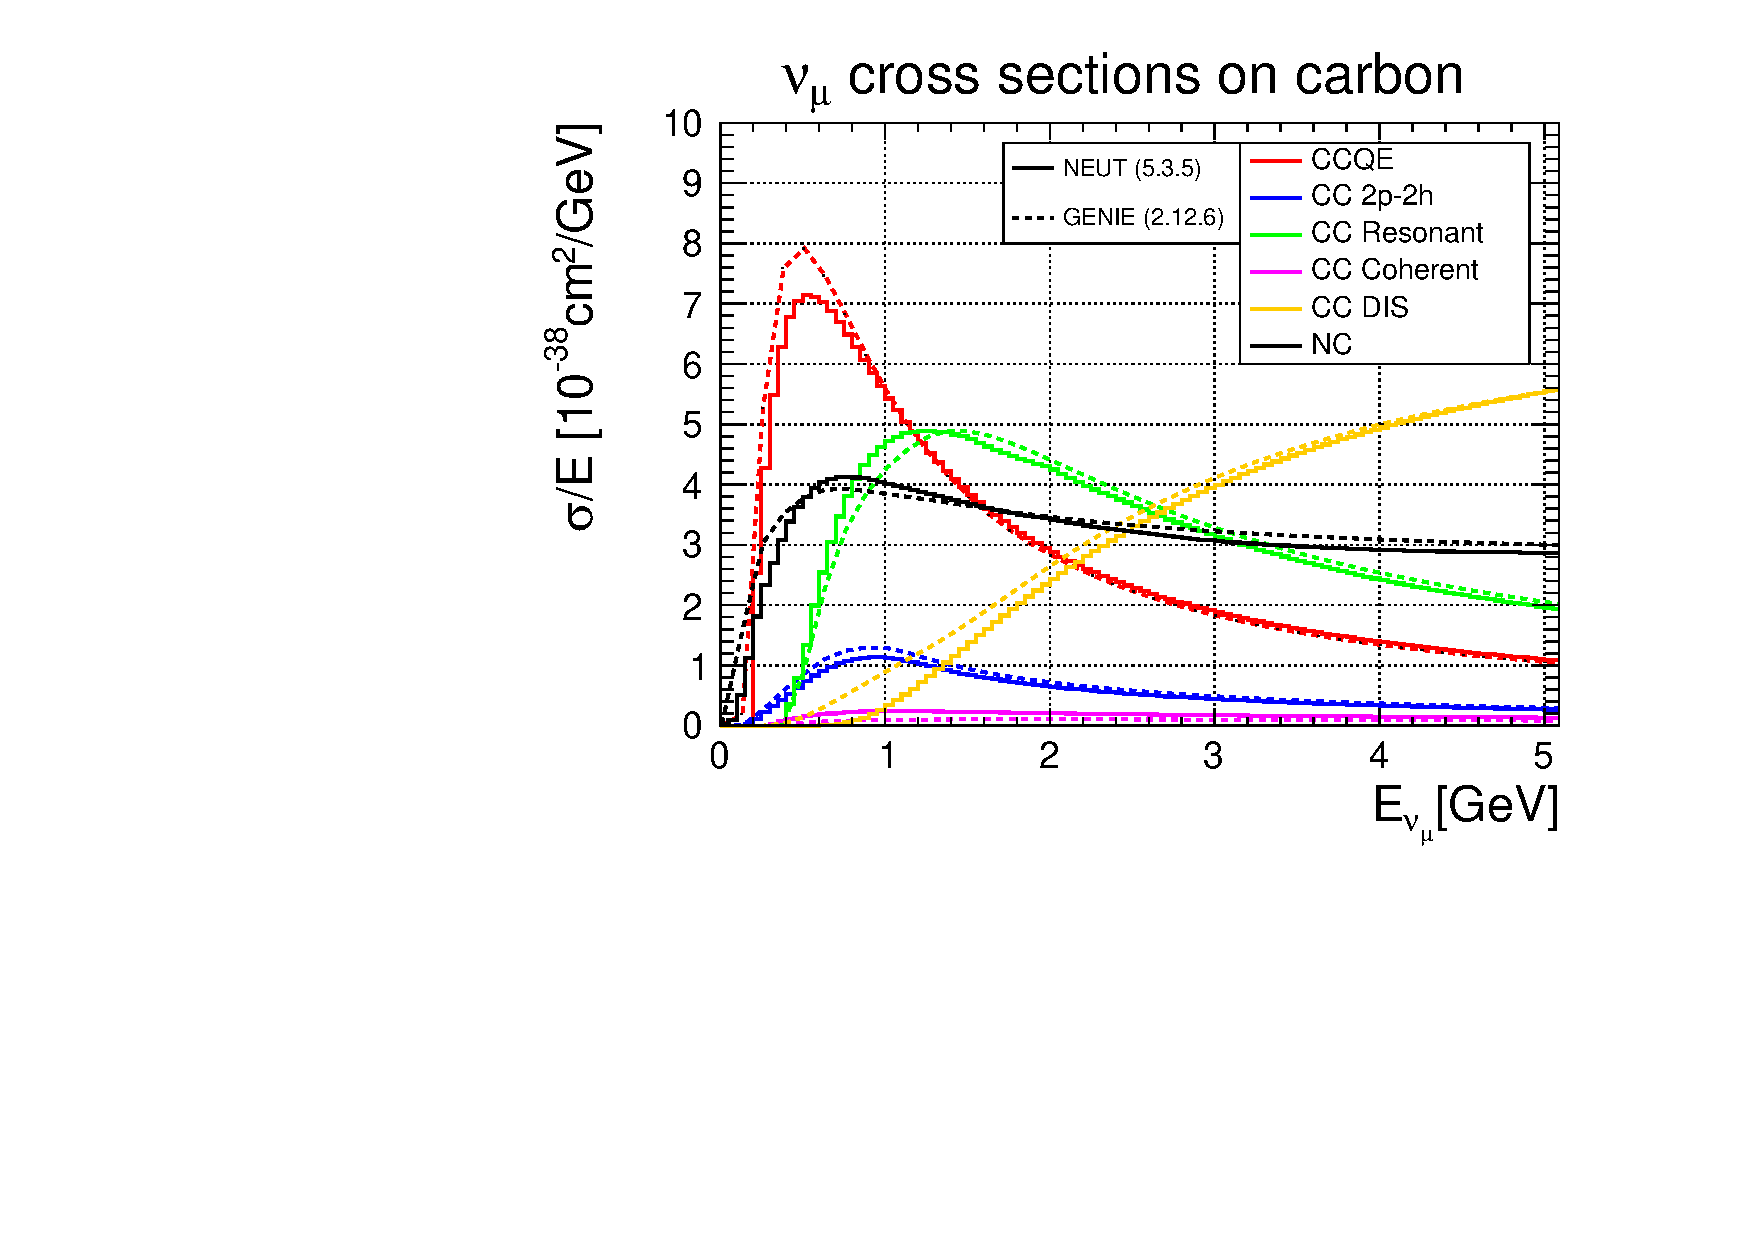
\includegraphics[width=0.7\textwidth]{images/Intro/cross_sections.pdf}
  \caption[Muon neutrino cross sections on carbon from GENIE and
  NEUT]{Muon neutrino cross sections on carbon from
    \Gls{GENIE}~\cite{GENIE1,GENIE2} and \Gls{NEUT}~\cite{NEUT}.}
  \label{fig:xsecs_plot}
\end{figure}

\subsection{Nuclear Model}
The nuclear model is purely related to the description of the nucleus,
it can be accessed via experiments such as electron scattering. One of
the most fundamental input to the nuclear model is the distribution of
momentum of the nucleons in the nucleus. There are several ways to
simulate this. The simplest of which is the Global Relativistic Fermi
Gas (\Gls{RFG}). In this model, the nucleons momentum simply follow a
Fermi distribution (the momentum of the nucleons is a quadratic
distribution up to the Fermi momentum, $p_F$), where the nuclear
matter is assumed to have a constant density, this is the default
model in \Gls{NEUT}, which is the neutrino interaction generator used
at \Gls{TK}.

The other model that was included in the \Gls{TK} simulations is the
Spectral Function (\Gls{SF}) model~\cite{Benhar}. In this model, all
the nucleon-nucleon interactions are factorised-out to produce a more
realistic distribution of the nucleon momentum in the nucleus. Note
that this model was significantly improved since its implementation in
the \Gls{NEUT} generator~\cite{Rocco:2016vyz}.

The \Gls{NEUT} \Gls{SF} models has proven to be insufficient to
predict \Gls{MINERVA} and \Gls{MiniBooNE} data~\cite{CallumFit}, so
the \Gls{RFG} model is used.

\subsection{Charged-Current Quasi-Elastic process}
\label{subsec:ccqe}
A Charged-Current Quasi-Elastic (\Gls{CCQE}) interaction is depicted
on the top left of Figure~\ref{fig:xsecs_diag}. In this process, a
(anti-) neutrino of a given flavour interacts with a single neutron
(proton) to create a negatively (positively) charged lepton of the
same flavour. These interactions can happen on free nucleon (hydrogen)
or nuclear target (carbon, oxygen), if the neutrino has enough energy
to create a charged lepton. The neutrino interacts via $W$-boson
exchange.

Since this is a two body process, momentum and energy conservation
laws can be used to reconstruct the energy of the neutrino. In the
case of a free nucleon, the reconstructed neutrino energy,
$E_\text{rec}$, is~\cite{MartiniERec}:
\begin{equation}
\label{eq:ereco}
E_{\text{rec}}=\frac{E_\text{l}-m_\text{l}^2/(2M)}
{1-\left(E_\text{l}-P_\text{l}\cos\left(\theta_\text{l}\right) \right)/M}
\end{equation}
where $E_\text{l}$ is the energy of the lepton (muon or electron),
$m_\text{l}$ is the lepton mass, $P_\text{l}$ its momentum,
$\cos\left(\theta_\text{l}\right)$ is the cosine of the lepton
scattering angle, and M is the mass of the struck nucleon (neutron for
neutrino and proton for anti-neutrino).

As can be seen in Figure~\ref{fig:xsecs_plot}, which shows the
neutrino cross section against its energy, the \Gls{CCQE} cross
section is largely dominant around 600~MeV, which is also the \Gls{TK}
peak energy. As will be described later, this is not a coincidence.

The formalism to calculate the value of the cross
section~\cite{LlewellynSmith} in the context of bubble chamber
experiments~\cite{ANLCCQE,BNLCCQE,CERNCCQE}. Most of the parameters
involved in the calculation of the cross section can be accessed via
electron scattering, however the cross section also depends on a
fundamental parameter which can only by accessed via neutrino
measurements, called the axial mass ($M_A^{QE}$).

The \Gls{CCQE} cross section is proportional to the following form
factor (so-called dipole form factor):
\begin{equation}
  \label{eq:ccqeff}
  F_A(Q^2) = \frac{g_A}{\left(1+\frac{Q^2}{M_A^{\text{QE~}2}}\right)^2}
\end{equation}
This form factor and $M_A^{QE}$ parameter are related to the spacial
extension of the nucleon for neutrino interactions by a inverse
Fourier transform. This has recently come into more focus as a dipole
form facbintor may not be justified for the neutrino
case~\cite{PhysRevD.93.113015,PhysRevD.92.113011}.

The description of the cross section quickly becomes more complicated
in the case of nuclear targets or even for
deuteron~\cite{SinghDeuteron}. In this case, corrections of various
kinds have to be applied~\cite{SmithMoniz,NievesCCinc}. Some of these
corrections are listed here:

\begin{itemize}
\item The nucleons have a binding energy in the nucleus, the
  consequence is that the excited nucleon after neutrino interaction
  has to have a over the Fermi energy to happen. If the excited
  nucleon does not go over this threshold, the event said to be Pauli
  blocked.
\item As was seen in the previous section, the nucleons move in the
  nucleus, the descriptions of the distribution of the nucleon
  momentum range from simple Global Relativistic Fermi Gas (\Gls{RFG})
  to more complex Spectral Functions~\cite{Benhar} or Local Fermi Gas
  (\Gls{LFG}).

  It is clear that depending on the nuclear model used, one will get
  different energy distributions for the initial state of the system
  just before the neutrino interaction. These models will produce
  different kinematics for the outgoing particle and ``Pauli block''
  different events.
\item The long range correlations has effect on $Q^2$ (which is the
  absolute value of the 4-momentum transfer squared): at low $Q^2$ the
  cross section is expected to be reduced; whereas it is enhanced at
  intermediate $Q^2$ and goes back to unity for
  $Q^2\rightarrow \infty $.  This correction, also refered as ``Random
  Phase Approximation'' (\Gls{RPA})~\cite{NievesCCinc} is due to the
  fact that the $W$-boson creates virtual particle-holes in the
  nuclear medium in which it is propagating.
\end{itemize}

It should be noted that most of our knowledge in the \Gls{CCQE} cross
section stems from bubble chamber
data~\cite{ANLCCQE,BNLCCQE,CERNCCQE}. Nuclear targets experiments such
as \Gls{MINERVA}~\cite{MinervaNuCCQE},
\Gls{MiniBooNE}~\cite{MiniBooNENuCCQE} and, in a lesser extent,
\Gls{TK}~\cite{T2KCCQE} and \Gls{K2K}~\cite{K2KCCQE} near detectors
data are still challenging to interpret. One of the reasons being that
these measurements cannot disentangle the multi-nucleon processes from
the pure \Gls{CCQE} contributions~\cite{CallumFit}. Indeed, all the
\Gls{CC}$0\pi$\footnote{\Gls{CC} with no pion in the final state
  measurements, as opposed to direct measurements of the \Gls{CCQE}
  measurements, includes events where pions are created in the nucleus
  but do not exit the nucleus, or events where several nucleons escape
  the nucleus.} measurements on nuclear targets show that the data is
higher than the one would get by only considering the \Gls{CCQE} cross
section. This hints towards the presence of another contribution.

\subsection{Multi-nucleon processes}
Multi-nucleon processes, also called ``np-nh'' for n-particles n-holes
(or even sometimes loosely referred as Meson Exchange Current
(\Gls{MEC})) are those processes where the neutrino interacts with a
correlated pair of nucleons. The cross section for these events to
happen is smaller than one for \Gls{CCQE} processes as can be seen in
Figure~\ref{fig:xsecs_plot}. They also are largely more complex to
calculate and to measure. This makes them one of the primary focuses
in the neutrino cross section community.

Due to their similarity with pure \Gls{CCQE} events, these events lead
to an enhancement to the total number of expected \Gls{CC}$0\pi$
events as explained earlier. An example of one of the many
contributing Feynman diagrams for this cross section is shown in top
right of Figure~\ref{fig:xsecs_diag}, where the similarity with
\Gls{CCQE} processes is clearer. Three main calculations for the
multi-nucleon cross section were done recently
in~\cite{MartiniNpNh1,MartiniNpNh2}, \cite{NievesNpNh1,NievesNpNh2}
and \cite{AmaroNpNh1,AmaroNpNh2}.

Note that despite the similarity in topology with the pure \Gls{CCQE}
processes, the reconstructed energy in
Equation~\ref{eq:ereco}~\cite{MartiniERec} does not hold for these
events since this is no longer a two body process.

np-nh events are by definition nuclear processes which can only be
accessed by modern neutrino experiments using a nuclear target, and
the corrections listed in the previous section need to be applied to
reliably calculate its cross section. Most of the knowledge on these
processes originates from experiments such as \Gls{K2K}~\cite{K2KCCQE}
and \Gls{MiniBooNE}~\cite{MiniBooNENuCCQE,MiniBooNEANuCCQE}, which
were the first to see the effect of these processes (enhancement of
the \Gls{CC}$0\pi$ cross section); these were followed a few years
later by \Gls{TK}~\cite{T2KCCQE}. More recently, the \Gls{MINERVA}
experiment released data which proves that our understanding of this
cross section is still very limited~\cite{minervaq3q0}. This
measurement shows that one needs to multiply the np-nh cross section
by a factor of two to fit the data. This is still a puzzle, which no
nuclear theorist has been able to explain yet.

The way to shed light on these processes will probably come from the
observation of the protons exiting the nucleus, with use of the
precise detectors in the Fermilab Short Baseline Neutrino
program~\cite{SBN,microboone}, although the theoretical calculations
of proton kinematics are still at their early
stage~\cite{MartiniProtonKine} (for example they are only available
for carbon and do not include interactions of the exiting protons with
the nuclear medium).



\subsection{Resonant processes}
\label{subsec:res}
\begin{figure}[ht]
  \center
  \hspace{1cm}\begin{fmffile}{feynmandiag/qsqw}
    \begin{fmfgraph*}(27,27)
      \fmfstraight
      \fmftop{i2,o3}
      \fmfleft{i1,b2,b3,i2}
      \fmfright{o1,o2,bo1,bo2,o3}
      \fmfbottom{i1,o1}
      \fmf{fermion,tension=1.5}{i2,v1}
      \fmflabel{$\nu$}{i2}
      \fmf{fermion}{v1,o3}
      \fmflabel{$l$}{o3}
      \fmf{fermion}{i1,v2}
      \fmflabel{$n/p$}{i1}
      \fmf{photon,label=$Z^0/W$}{v1,v2}
      \fmf{fermion,tension=0.5}{v2,o2}
      \fmflabel{$X, W_{inv}$}{o2}
      \fmf{fermion,tension=0.5}{v2,o1}
      \fmffreeze
      \fmfcmd{style_def marrowQ expr p = drawarrow subpath (1/4, 3/4) of p shifted 6 right
        withpen pencircle scaled 0.4; label.top(btex $Q^2$ etex, point 0.5 of p
        shifted 15 right shifted 6 down); enddef;}
      \fmf{marrowQ}{v1,v2}
    \end{fmfgraph*}
  \end{fmffile}
  \vspace{0.3cm}
  \caption[Illustration of the $Q^2$ and $W_{inv}$ quantities for a
  generic neutrino reaction]{Illustration of the $Q^2$ and $W_{inv}$
    quantities for a generic neutrino reaction. $l$ denotes a charged
    lepton or a neutrino of the same flavour as the incoming one
    ($\nu$), depending on whether the interaction is Charged-Current
    ($W$) or Neutral-Current ($Z^0$). The $X$ denotes any particle(s)
    of total energy $W_{inv}$ that has been generated by the boson
    interaction on a nucleon. In the case of a resonant interaction,
    the $X$ would be a nuclear resonance that decays into a pion or a
    photon, and a nucleon.}
  \label{fig:FeynmanQ2W}
\end{figure}

A Charged-Current Resonant (\Gls{CC}\Gls{RES}) process is illustrated
in the middle left of the Figure~\ref{fig:xsecs_diag}. In the case of
a resonant interaction, rather than interacting ``elastically'' with a
nucleon, the $W$-boson has enough energy to create a ``nuclear
resonance,'' which, in simple terms, can be seen as equivalent to
flipping the spin of a valence quark in the proton, and changing the
isospin of one or several of the quarks. The resonance usually
undergoes a strong decay by emitting of a pion and a nucleon. The
resonance created is a much more complex object than a simple Dirac
spinor and the calculation of the amplitudes of this cross section is
more involved mathematically than in the case of
\Gls{CCQE}~\cite{Rein1,Rein2}.

These \Gls{RES} cross sections are usually parametrised by a
double differential cross section of the form
$\frac{d^2\sigma}{dQ^2dW_{inv}}$, where $Q^2$ is the absolute value of
the 4-momentum transfer squared and $W_{inv}$ is the invariant mass of
the outgoing hadron system. These quantities are illustrated in
Figure~\ref{fig:FeynmanQ2W}.

Some additional corrections due to the nuclear environment have to be
taken into account for reliable cross section predictions. The main of
which are the Final State Interactions (\Gls{FSI}). These affect the
exiting pions and can change the topology of the events if a pion is
absorbed, for example. Another correction can be applied on the
resonance, since it can also scatter with a nucleon during its very
short life-time. This leads to processes such as pion-less delta
decays or a change in the decay width of the
resonance~\cite{Oset1987,Singh1998}.

Also, note that there exist several resonances ($\Delta_{1232}$ having
the lowest mass of them, and contributing the most to the amplitude)
and a non-resonant ``background''~\cite{Background} (where the nucleon
is used as a propagator between the interacting boson and the decay to
pion and nucleon). These different contributions produce the same
final states and the amplitudes for each of them needs to be added
coherently to correctly take into account interferences. These
interferences can significantly modify the topology of the single pion
events~\cite{Minoo}.

As it was the case for \Gls{CCQE}, most of the models are constrained
by the bubble chamber experiments~\cite{ANLPion,ANLNCPion,BNLPion},
although there is still some confusion in the compatibility between
these data sets~\cite{Wilkinson:2014yfa}. The
\Gls{MINERVA}~\cite{MINERvACCPion},
\Gls{MiniBooNE}~\cite{MiniBooNECC1PiP,MiniBooNECC1Piz,MiniBooNENCPi0},
\Gls{K2K}~\cite{K2KPion} and \Gls{TK} data are still a long way from
being understood within an unique framework.

\subsection{Deep Inelastic Scattering processes}
The Deep Inelastic Scattering (\Gls{DIS}) processes occur at higher
energies when the $W$-boson interacts with a single quark. The process
is illustrated in Figure~\ref{fig:xsecs_diag} (bottom right). In DIS
events, many pions are usually created.

This process can be calculated from first principles but relies on the
precise knowledge of the parton distribution functions, at low $Q^2$
and relatively high $x$\footnote{$Q^2$ is the momentum transfer of the
  probe to the target, and $x$ is defined as $\frac{Q^2}{2M\omega}$,
  where M is the target mass (if at rest) and $\omega$ is the energy
  transfer.\label{ftn:qsquare}} regions, for which scaling violations
occurs and DGLAP equations, which are used to extrapolate \Gls{PDF}
across $Q^2$, do not hold~\cite{DGLAP1,DGLAP2,DGLAP3,DGLAP4}.

Most of the data used for the \Gls{PDF} (Parton Distribution
Functions) fits come from \Gls{NuTEV}~\cite{nutev},
\Gls{CHORUS}~\cite{chorus} and \Gls{CDHSW}~\cite{CDHSW}. From these,
it is still unclear whether coupled \Gls{DIS}~/~nuclear effects such
as the \Gls{EMC} effect or the \gls{anti-shadowing} happen for
neutrino interactions. These phenomena are observed in \Gls{DIS}
electron scattering: it was shown that the nuclear cross section is
enhanced in certain regions of $x$ compared to the one of the free
nucleon. They have unclear theoretical explanations.

Some more recent data from \Gls{MINERVA}~\cite{Mousseau} is hinting
towards the same conclusion (absence of anti-shadowing effect).

For the hadronisation physics, it was recently noted that the
\Gls{HERMES} data~\cite{HERMES} could used to better predict some
basic quantities related to hadron
multiplicities~\cite{Katori:2014fxa}.

These processes need to be carefully studied in the context of higher
energy beams, such as the \Gls{DUNE}~\cite{DUNE1,DUNE2,DUNE3,DUNE4}
one, or \Gls{NOvA}~\cite{Ayres:2007tu} and atmospheric neutrino
experiments~\cite{Aartsen:2014oha}.

\subsection{Shallow Inelastic Scattering processes}
Between the \Gls{RES} and \Gls{DIS}, other processes called Shallow
Ineslastic Scattering processes can happen. This is refered
theoretically as the ``transition region.'' These processes are added
because the regions of validity of the \Gls{RES} and \Gls{DIS} cross
sections are disjoint. In practice, the problem is overcome by using
the continuum (background term) of the \Gls{RES} cross section and
ensuring continuity in the $W$ variable~\cite{GENIE1}.

Although these channels are very important in the context of
\Gls{NOvA} (because the neutrino energy distribution peaks at 2~GeV),
there are still little theoretical calculations. A last notable
reference is a two pions neutrino production calculation
in~\cite{Hernandez:2007ej}.

\subsection{Coherent pion production processes}
The coherent processes happen when the $W$-boson from the neutrino has
a very low momentum and cannot resolve individual nucleons inside the
nucleus~\cite{Rein:2006di,Berger:2008xs}. In that case, the boson
interacts with the whole nucleus. A pion is created from de-excitation
of the nucleus and critically, this pion does not undergo final state
interactions. Only recent nuclear data is sensitive to the coherent
pion production processes, historical measurements date from 1988 with
the experiments SKAT, BEBC, CHARM-II and
E632~\cite{Grabosch:1985mt,Allport:1988cq,Vilain:1993sf,Aderholz:1988cs},
that measured neutrino coherent pion production on neon. More modern
experiments also tried to measure the coherent interaction on plastic
scintillator, at the beginning unsuccessfully
(\Gls{K2K}~\cite{Hasegawa:2005td} and
\Gls{SciBooNE}~\cite{PhysRevD.78.112004}). The first charged-current
measurement on plastic scintillator was made by
\Gls{MINERVA}~\cite{Higuera:2014azj}, and was followed by
\Gls{TK}~\cite{Abe:2016fic}. \Gls{ArgoNeuT}~\cite{Acciarri:2014eit}
also measured these interactions on liquid argon.

\subsection{Electron neutrino cross sections}
\label{subsec:electronnu}
Electron neutrino cross sections have the same contributing Feynman
diagrams as the ones shown in Figure~\ref{fig:xsecs_diag}. There are
further differences expected since the fact that electrons have a
smaller mass than muons opens phase space when one compares muon
neutrino to electron neutrino cross sections. Further complications
arise for the so-called Second Class Current (\Gls{SCC}) and radiative
corrections~\cite{Day:2012gb}. The electron neutrino cross section in
these energies always suffers from having very low statistical power
(few events), since it is simpler to create an muon neutrino beam as
will be seen later (Section~\ref{sec:t2kbeamline}). The current
knowledge stems from bubble chamber experiments
(Gargamelle~\cite{Blietschau:1977mu}), \Gls{TK}~\cite{nueT2K} and
\Gls{MINERVA}~\cite{Wolcott:2015hda}. There has not been an exclusive
measurement of electron anti-neutrino cross section made on its own
yet.

\subsection{Anti-neutrino cross sections}
Anti-neutrino cross sections are also a challenge because their cross
section is about half of the neutrino ones. This happens because a
cancellation appears in the matrix element of the anti-neutrino cross
section due to the presence of the anti-neutrino.

Some experiments, such as \Gls{MiniBooNE} and \Gls{MINERVA} have been
exposed to anti neutrino beams and have made measurement of the
\Gls{CCQE} and \Gls{CC}1$\pi$ cross
sections~\cite{AguilarArevalo:2013dva,Fields:2013zhk,Aliaga:2015wva}.

\subsection{Neutral-Current processes}
All the cross sections described earlier have their equivalent in the
Neutral Current (\Gls{NC}) channel. However, it is much harder to
detect these processes due to the absence of a high energy lepton.

\subsubsection{Neutral-Current elastic process}
The \Gls{CCQE} equivalent is the \Gls{NC} elastic process (sometime
referred as \Gls{NCEl}), which only produces a single proton (or a
neutron) after neutrino interaction. As for \Gls{CCQE}, the
nucleon-level information mostly comes from bubble chamber
experiments~\cite{Ahrens:1986xe,Garvey:1992cg,Alberico:1998qw}.
% These measurements have been used to determine the strange form
% factors (so called $\Delta s$ factor of the proton), which can be
% accessed at $Q^2 \rightarrow 0$~\cite{Garvey:1993sg}; and the weak
% angle, $\sin^2\theta_{W}$.  More recently, the \Gls{MiniBooNE}
% collaboration used its data on oil target to measured the $\Delta s$
% parameter~\cite{AguilarArevalo:2010cx,AguilarArevalo:2013nkf},
% although there are now very strong concerns about the
% parametrisation at low $Q^2$ due to the \Gls{RPA} correction.

\subsubsection{Neutral-Current neutral pion processes}
Another channel of interest is the \Gls{NC}1\gls{piz}, which leads to
production of two photons via the \gls{piz} decay. In the case when
one of the photon has a low energy, it is very common to interpret
these events as electron neutrino interaction, since both of them
create electro-magnetic (\Gls{EM}) showers in the Cherenkov detectors.
Indeed, the photons, in the energy range of 100~MeV to 5~GeV interact
via Compton scattering and create electron~/~positron pairs. At
similar energies, electron loose energy by Cherenkov and
bremsstrahlung~\cite{PDG2014} processes. All these interactions
involve creation and excitation of electrons and positrons and
therefore create the same signal.

This was already a problem at \Gls{K2K} which used the water Cherenkov
Kamiokande detector as far detector. To overcome this problem, the
collaboration use its near $1$~ton Cherenkov detector was used to
measure this channel~\cite{Nakayama:2004dp}. \Gls{MiniBooNE} later
measured this same channel for neutrino and
anti-neutrino~\cite{AguilarArevalo:2009ww}. The equivalent coherent
process were also measured by the
\Gls{MiniBooNE}~\cite{AguilarArevalo:2008xs} and by the
\Gls{NOMAD}~\cite{KULLENBERG2009177} collaborations.

\subsubsection{Neutral-Current single photon processes}
\label{subsubsec:ncgprocesses}
The channel of interest of this thesis is the ``\Gls{NC} gamma,'' or
\nisp. In this process, a single photon is created after the neutrino
interaction. The phenomenology will be described in greater details in
a subsequent chapter (Chapter~\ref{chap:pheno}). Note that there is
currently no observation of this process. The only search that was
ever done was conducted in the \Gls{NOMAD}
detector~\cite{NOMADncg}. For the same reason as the one described in
the previous paragraph (similar photon and electron topology in
detectors), the interest in this channel is increasing.

\subsubsection{Neutral-Current diffractive processes}
Very recently, \Gls{MINERVA} reported an unexplained excess of neutral
pion-like events. Observations seem to hint towards the presence of a
diffractive channel on hydrogen atom~\cite{Wolcott:2016hws}. They have
the same topology as the coherent events (i.e. very forward). However,
a clear theoretical interpretation is still lacking. The observed
cross section is small
($0.26\pm0.02\text{(stat)}\pm0.08\text{(syst)}\times10^{39}$ on
hydrocarbon target~\cite{Wolcott:2016hws}). It should be noted that
these events are not in the neutrino interaction generators
\Gls{NEUT}~\cite{NEUT} and \Gls{GENIE}~\cite{GENIE1,GENIE2} used for
\Gls{TK} analyses.










